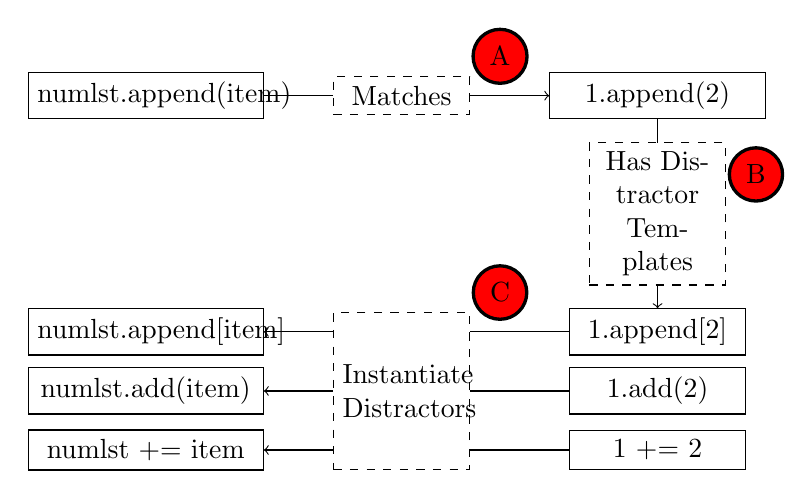
\begin{tikzpicture}[node distance=2cm]

    \node (line) [draw, text width=2.75cm, align=center] {numlst.append(item)};
    \node (extract) [draw, xshift=4.5cm, right of=line, text width=2.5cm, align=center] {\boxed{1}.append(\boxed{2})};

    \node (d1struct) [draw, yshift=-1cm, below of=extract,    text width=2cm, align=center]   {\boxed{1}.append[\boxed{2}]};
    \node (d2struct) [draw, yshift=1.25cm, below of=d1struct, text width=2cm, align=center] {\boxed{1}.add(\boxed{2})};
    \node (d3struct) [draw, yshift=1.25cm, below of=d2struct, text width=2cm, align=center] {\boxed{1} += \boxed{2}};

    \node (d1) [draw, yshift=-1cm, below of=line, text width=2.75cm, align=center] {numlst.append[item]};
    \node (d2) [draw, yshift=1.25cm, below of=d1, text width=2.75cm, align=center]       {numlst.add(item)};
    \node (d3) [draw, yshift=1.25cm, below of=d2, text width=2.75cm, align=center]       {numlst += item};

    % Arrows
    \draw[->] (line.east) -- (extract.west);
    \draw[->] (extract) -- (d1struct);
    \draw[->] (d1struct.west) -- (d1.east);
    \draw[->] (d2struct.west) -- (d2.east);
    \draw[->] (d3struct.west) -- (d3.east);

    % Transition labels
    \node (matches) [fill=white, xshift=1.25cm, right of=line, draw, text width=1.5cm, align=center, dashed] {Matches};
    \node (hasdist) [fill=white, yshift=0.5cm, below of=extract, draw, text width=1.5cm, align=center, dashed] {Has Distractor Templates};
    \node (instantiate) [text centered, fill=white, xshift=-1.25cm, left of=d2struct, draw, text width=1.5cm, minimum height=2cm, dashed] {Instantiate\\ Distractors};

    % Labels
    \node (1) [draw, circle, right of=matches,     fill=red, very thick, xshift=-0.75cm, yshift=0.50cm] {A};
    \node (2) [draw, circle, right of=hasdist,     fill=red, very thick, xshift=-0.75cm, yshift=0.50cm] {B};
    \node (3) [draw, circle, right of=instantiate, fill=red, very thick, xshift=-0.75cm, yshift=1.25cm] {C};


\end{tikzpicture}

